%\RequirePackage[pagewise]{lineno}
%\documentclass[11pt, letterpaper,]{article}
\documentclass[prl,preprint]{revtex4}
%\documentclass[rmp,linenumbers,preprint]{revtex4}
\usepackage{amssymb,amsfonts,amsmath}
%\usepackage{setspace}
%\usepackage[top=25mm, bottom=25mm, left=25mm, right=25mm]{geometry}
%\bibpunct{(}{)}{;}{author-year}{}{,} 
%\doublespacing
%\bibliographystyle{genetics}

\usepackage{graphicx}
\usepackage{amsmath}
\usepackage{natbib}

\newcommand{\EQ}[1]{Eq.~(\ref{eq:#1})}
\newcommand{\EQS}[2]{Eqs.~(\ref{eq:#1}) and (\ref{eq:#2})}
\newcommand{\FIG}[1]{Fig.~\ref{fig:#1}}
\newcommand{\TAB}[1]{Tab.~\ref{tab:#1}}
\newcommand{\REF}[1]{ref.~\citep{#1}}

\newcommand{\beast}[1]{\emph{#1}}
\newcommand{\gene}[1]{\emph{#1}}
\newcommand{\x}{x}
\newcommand{\xs}{\bar{\x}}
\newcommand{\xz}{z}
\newcommand{\xzs}{\bar{\xz}}
\newcommand{\dx}{\delta \x}
\newcommand{\n}{n}
\newcommand{\rate}{\gamma}
\newcommand{\ns}{\bar{\n}}
\newcommand{\dn}{\delta \n}
\newcommand{\mk}{\bar{k}}
\newcommand{\dk}{\delta \bar{k}}
\newcommand{\tx}[1]{\xz_{#1}}
\newcommand{\mr}[1]{\psi^{(#1)}}
\newcommand{\ml}[1]{\phi^{(#1)}}
\newcommand{\Smin}{S^*}
\newcommand{\mut}{u}
\newcommand{\cp}{\iota}

%DSF ADDED
\newcommand{\pr}{{\rm Prob}}
\newcommand{\pd}[2]{\frac{\partial #1}{\partial #2}}
\newcommand{\la}{\langle}
\newcommand{\ra}{\rangle}
\newcommand{\gr}{\theta}
%%%%

\begin{document}
\title{Supplement -- Fluctuations of fitness distributions and the rate of Muller's ratchet}
\author{R.~A.~Neher}
\affiliation{Max-Planck Institute for Developmental Biology, T\"ubingen, 72070, Germany}
\author{B.~I.~Shraiman}
\affiliation{Kavli Institute for Theoretical Physics and Department of Physics, University of California, Santa Barbara, CA 91306}
%${}^{*}$Kavli Institute for Theoretical Physics, \\${}^{\ddagger}$Department of Physics, University of California, Santa Barbara, CA 91306 and \\${}^{\dagger}$Max-Planck Institute for Developmental Biology, T\"ubingen, 72070, Germany}
\date{\today}
\maketitle



%\onecolumngrid
To analyze the covariances of different fitness classes, we begin with Eq.~(7) of the main text, which expresses $\dx_k(\tau)$ in terms of eigenvectors $\dx_k(\tau) = \sum_j \mr{j}_k a_j(\tau)$. Projecting on the left eigenvectors then results in equations for $a_j(\tau)$
\begin{equation}
\label{eq:modes}
\frac{d}{d\tau} a_j(\tau) = -j a_j(\tau) + \sum_k \ml{j}_k \sqrt{\frac{\xs_k}{Ns}} \eta_k(\tau)
\end{equation}
where $\eta_k(\tau)$ are uncorrelated Gaussian white noise terms with $\la \eta_k(\tau) \eta_l(\tau')\ra = \delta_{kl}\delta(\tau-\tau')$. Since each noise term $\eta_k$ contributes to all $a_j$, the noise induces correlated fluctuations of the $a_j(\tau)$, which we need to understand in order to analyze the fluctuations of the fitness distributions. The inhomogeneous \EQ{modes} has the  solution
\begin{equation}
a_j(\tau) = \int_{-\infty}^{\tau}d\tau' e^{-j(\tau-\tau')} \sum_k \ml{j}_k \sqrt{\frac{\xs_k}{Ns}} \eta_k(\tau')
\end{equation}
The autocorrelation function of the loadings of different eigendirections separated by $\Delta \tau$ in time is therefore given by
\begin{equation}
\begin{split}
\langle a_i(\tau) a_j(\tau+\Delta\tau)\rangle &= \int_{-\infty}^\tau d\tau'\int_{-\infty}^{\tau+\Delta\tau} d\tau'' e^{-i(\tau-\tau')-j(\tau+\Delta\tau -\tau'')}\sum_{k,l} \frac{\ml{i}_k\ml{j}_l\sqrt{\xs_k\xs_l}}{Ns} \langle \eta_k(\tau')\eta_l(\tau'')\rangle\\
&=  \int_{-\infty}^\tau d\tau' e^{-i(\tau-\tau')-j(\tau+\Delta\tau -\tau')}\sum_{k} \frac{\ml{i}_k\ml{j}_k\xs_k}{Ns}\\
&= \frac{e^{-j\Delta\tau}}{i+j}\sum_{k} \frac{\ml{i}_k\ml{j}_k\xs_k}{Ns}
\end{split}
\end{equation}
where we have used $\la \eta_k(\tau) \eta_l(\tau')\ra = \delta_{kl}\delta(\tau-\tau')$.

\subsection*{Correlation functions $n_0$ and the mean}
To calculate the variances and covariance of $\x_0$ and the mean fitness, we express them in terms of the eigenmodes $a_j(\tau)$ ($j>0$)
\begin{eqnarray}
\dx_0(\tau) &=& \sum_{j>0} \mr{j}_0 a_j(\tau)  = e^{-\lambda} \sum_{j>0} a_j(\tau)\\
\dk(\tau) &=& \sum_{j>0,k} k\mr{j}_k a_j(\tau) = \sum_{j>0,k} k(\xs_{k-j}-\xs_k) a_j(\tau) =  \sum_{j>0} j a_j(\tau)
\end{eqnarray}

\subsection*{The auto-correlation of $\x_0$}
The auto-correlation of $\x_0$ is given by
\begin{equation}
\label{eq:n0var}
\begin{split}
\la \x_0(\tau) \x_0(\tau+\Delta\tau)\ra &=  e^{-2\lambda} \sum_{i,j>0} \frac{e^{-j\Delta\tau}}{i+j}\sum_{k} \frac{\ml{i}_k\ml{j}_k\xs_k}{Ns} \\
& = \frac{e^{-\lambda}}{Ns} \sum_{i,j>0} \frac{\lambda^{i+j}e^{-j\Delta\tau}}{i+j}\sum_{k=0}^{\min(i,j)} \frac{(-1)^{i+j}\lambda^{-k}}{(j-k)!(i-k)!k!} \\
& = \frac{e^{-\lambda}}{Ns} \int_0^\infty dz \sum_{i,j>0} e^{-z(i+j)}\lambda^{i+j}e^{-j\Delta\tau}\sum_{k=0}^{\min(i,j)} \frac{(-1)^{i+j}\lambda^{-k}}{(j-k)!(i-k)!k!} 
\end{split}
\end{equation}
Let us focus on the triple sum inside the integral and simplify it by introducing $a=-\lambda e^{-z}$ and $b=-\lambda e^{-z-\Delta\tau}$. Furthermore, let us look at the $i=j$ and the $i\neq j$ contributions separately. The diagonal contribution  ($i=j$) is
\begin{equation}
\begin{split}
&\sum_{i=0} a^ib^i \sum_{k=0}^{i} \frac{\lambda^{-k}}{(i-k)!(i-k)!k!} = \sum_{i>0} \sum_{k=0}^{i} \frac{(ab)^{i-k}(ab)^{k}\lambda^{-k}}{k!((i-k)!)^2}\\
&=\sum_{k>0} \sum_{i\geq k} \frac{(ab)^{i-k}(ab)^{k}\lambda^{-k}}{k!((i-k)!)^2} + \sum_{i>0} \frac{(ab)^{i}}{(i!)^2} \\
&=\sum_{k>0} \frac{(ab)^{k}\lambda^{-k}}{k!}\sum_{n\geq 0} \frac{(ab)^{n}}{(n!)^2} + J_0(-\cp 2\sqrt{ab})-1   \quad\quad \mathrm{using}\quad n=i-k\\
&=(e^{ab/\lambda}-1)J_0(-\cp 2\sqrt{ab}) + J_0(-\cp 2\sqrt{ab})-1\\
&=e^{ab/\lambda} J_0(-\cp 2\sqrt{ab})-1
\end{split}
\end{equation}
where $J_n(z)$ is the $n$th Bessel function of first kind, and $\cp=\sqrt{-1}$. 
When evaluating the off-diagonal contribution, we will encounter terms like
\begin{equation}
\sum_{k>0} \frac{(ab)^{k}}{k!(k+m)!} = \sum_{k} \frac{(ab)^{k}}{k!(k+m)!} - \frac{1}{m!} = \frac{J_m(2\cp\sqrt{ab})}{(\cp\sqrt{ab})^m}-\frac{1}{m!}
\end{equation}
The off-diagonal contribution can be further split into the parts $i>j$ and $i<j$ which can be evaluated as follows:
\begin{equation}
\begin{split}
&\sum_{0<i<j} a^{i}b^j\sum_{k\geq 0}^{i} \frac{\lambda^{-k}}{k!(j-k)!(i-k)!} 
= \sum_{i>0}\sum_{j>i} a^{i}b^{j-i+i}\sum_{k\geq 0}^{i} \frac{\lambda^{-k}}{k!(i+(j-i)-k)!(i-k)!}\\
& = \sum_{i>0}\sum_{m>0} a^{i}b^{m+i}\sum_{k\geq 0}^{i} \frac{\lambda^{-k}}{k!(i+m-k)!(i-k)!}  \quad\quad \mathrm{using}\quad m=j-i \\
&=\sum_{k>0}\sum_{m>0} \sum_{i\geq k} \frac{a^{i}b^{m+i}\lambda^{-k}}{k!(i+m-k)!(i-k)!} + \sum_{m>0} \sum_{i>0} \frac{a^{i}b^{m+i}}{(i+m)! i!} \\
&=\sum_{k>0}\sum_{m>0}\sum_{n\geq 0} \frac{ a^{n+k}b^{m+n+k}\lambda^{-k}}{k!(n+m)!n!} + \sum_{m>0} b^{m}\sum_{i>0} \frac{(ab)^{i}}{(i+m)! i!}  \quad\quad \mathrm{using}\quad n=i-k\\
&=\sum_{k>0}\sum_{m>0}\frac{ a^{k}b^{m+k}\lambda^{-k}}{k!}\frac{J_m(2\cp\sqrt{ab})}{(\cp\sqrt{ab})^m} + \sum_{m>0} b^{m}\left(\frac{J_m(2\cp\sqrt{ab})}{(\cp\sqrt{ab})^m} -\frac{1}{m!}\right)\\
&=\sum_{m>0}\sum_{k\geq 0}\frac{  a^{k}b^{k}b^{m/2}a^{-m/2}\lambda^{-k}}{k!}\frac{J_m(2\cp\sqrt{ab})}{(\cp)^m} -e^b+1 = \sum_{m>0} \left(\frac{b}{a}\right)^{m/2}e^{ab/\lambda}\frac{J_m(2\cp\sqrt{ab})}{(-1)^{m/2}} -e^b+1\\ &=e^{ab/\lambda}\sum_{m>0} \left(\frac{b}{a}\right)^{m/2}(-\cp)^m J_m(2\cp\sqrt{ab}) -e^b+1
\end{split}
\end{equation}
The off-diagonal terms for $i>j$ is obtained by interchanging $a$ and $b$ such that the full off-diagonal contribution is 
\begin{equation}
e^{ab/\lambda}\sum_{m>0} \left[\left(\frac{b}{a}\right)^{m/2}+\left(\frac{a}{b}\right)^{m/2}\right](-\cp)^m J_m(2\cp\sqrt{ab}) -e^a-e^b+2
\end{equation}
Next, we use the definition of the generating function of the Bessel functions (\citet{GR}, 8.511)
\begin{equation}
e^{\frac{1}{2}(t-t^{-1})z} =J_0(z) +  \sum_{m>0} (t^m+(-t)^{-m}) J_m(z) 
\end{equation}
which turns the off-diagonal contribution into 
\begin{equation}
e^{ab/\lambda}\left(e^{\sqrt{ab} \left(\sqrt{\frac{b}{a}}+\sqrt{\frac{a}{b}}\right)}-J_0(2\cp\sqrt{ab})\right)-e^a-e^b+2
\end{equation}
Combining the diagonal and off-diagonal contributions and substituting $a$ and $b$, we find for the integrand in \EQ{n0var}
\begin{equation}
e^{ab/\lambda+\sqrt{ab} \left(\sqrt{\frac{b}{a}}+\sqrt{\frac{a}{b}}\right)}-e^a-e^b+1 = 
e^{\lambda e^{-2z-\Delta \tau}-\lambda e^{-z} -\lambda e^{-z-\Delta \tau}}-e^{-\lambda e^{-z}}-e^{-\lambda e^{-z-\Delta \tau}}+1
\end{equation}
The auto-correlation of $\x_0$ is therefore given by
\begin{equation}
\begin{split}
\la \x_0(\tau) \x_0(\tau+\Delta\tau)\ra & = \frac{e^{-\lambda}}{Ns} \int_0^\infty dz \left(e^{\lambda e^{-2z-\Delta\tau}}e^{-\lambda(e^{-z}+e^{-z-\Delta\tau})}-e^{-\lambda e^{-z}}-e^{-\lambda e^{-z-\Delta\tau}}+1\right) \\
&= \frac{e^{-\lambda}}{Ns} \int_0^1 \frac{d\theta}{\theta} \left(e^{\lambda \theta^2 e^{-\Delta\tau} -\lambda\theta(1+e^{-\Delta\tau})}-e^{-\lambda \theta}-e^{-\lambda \theta e^{-\Delta\tau}}+1\right)
\end{split}
\end{equation}


\subsection*{Auto-correlation of the mean fitness}
The autocorrelation function of the mean is defined as
\begin{equation}
\begin{split}
\la \dk(\tau) \dk(\tau+\Delta\tau) \ra &= \sum_{i,j>0} ij \la a_i(\tau)a_j(\tau+\Delta\tau)\ra \\
&= \partial_\mu \partial_\nu \frac{1}{Ns} \int_0^\infty dz \sum_{i,j>0} \mu^i \nu^j e^{-z(i+j)}\lambda^{i+j}e^{-j\Delta\tau}\sum_{k=0}^{\min(i,j)} \frac{(-1)^{i+j}\lambda^{-k}}{(j-k)!(i-k)!k!}
\end{split}
\end{equation}
where the last line is to be evaluated at $\nu=\mu=1$. Hence the problem is reduced to the one already solved with $a=-\mu\lambda e^{-z}$ and $b=-\nu\lambda e^{-z-\Delta\tau}$. We find 
\begin{equation}
\begin{split}
\langle\dk(\tau) \dk(\tau+\Delta\tau )\rangle  %&= e^{\lambda} \int_0^1 \frac{d\theta}{\theta} \partial_\mu \partial_\nu\left(e^{\mu\nu \lambda \theta^2e^{-\Delta\tau } -\lambda(\nu+\mu e^{-\Delta\tau }) \theta}-e^{-\mu\lambda \theta}-e^{-\mu\lambda \theta e^{-\Delta\tau }}+1\right)\\
% & =e^{\lambda}\int_0^1 \frac{d\theta}{\theta} \partial_\mu \left(\mu \lambda \theta^2e^{-\Delta\tau }- \lambda \theta\right) e^{\mu\nu \lambda \theta^2e^{-\Delta\tau } -\lambda(\nu+\mu e^{-\Delta\tau }) \theta}\\
% & =e^{\lambda}\int_0^1 \frac{d\theta}{\theta} e^{\lambda \theta^2e^{-\Delta\tau } -\lambda(1+e^{-\Delta\tau }) \theta} \left(\lambda \theta^2e^{-\Delta\tau }  +\left(\lambda \theta^2e^{-\Delta\tau }- \lambda \theta\right)\left(\lambda \theta^2e^{-\Delta\tau }- \lambda e^{-\Delta\tau } \theta\right)\right) \\
 & =\frac{\lambda e^{\lambda}}{Ns}\int_0^1 d\theta e^{-\Delta\tau } e^{\lambda \theta^2e^{-\Delta\tau } -\lambda(1+e^{-\Delta\tau }) \theta} \left(\theta  +\lambda \theta\left(\theta e^{-\Delta\tau }- 1\right)\left(\theta- 1\right)\right)
 \end{split}
\end{equation}


\subsection*{Cross-correlation of $\x_0$ and the mean fitness}
When calculating the cross-correlation between $\x_0$ and the mean fitness we have to distinguish the cases where $\x_0$ precedes the mean fitness and vice-versa. Otherwise, the calculation proceeds almost unchanged from the cases discussed above.
\begin{equation}
\begin{split}
\la \x_0(\tau) \dk(\tau+\Delta\tau) \ra &= \sum_{i,j>0} j \la a_i(\tau)a_j(\tau+\Delta\tau)\ra \\
&= \partial_\nu \frac{1}{Ns} \int_0^\infty dz \sum_{i,j>0} a^i b^j\sum_{k=0}^{\min(i,j)} \frac{(-1)^{i+j}\lambda^{-k}}{(j-k)!(i-k)!k!}
\end{split}
\end{equation}
with $a=-\lambda e^{-z}$, $b=-\nu \lambda e^{-z-\Delta\tau}$ if $\Delta\tau>0$ and $a=-\lambda e^{-z+\Delta\tau}$, $b=-\nu \lambda e^{-z}$ if $\Delta\tau<0$. The result is 
\begin{equation}
\langle \dx_0(\tau) \dk(\tau+\Delta\tau)\rangle   = \frac{\lambda}{Ns} \begin{cases} 
  e^{-\Delta\tau} \int_0^1 d\theta \left((\theta-1)e^{e^{-\Delta\tau}\lambda \theta^2-\lambda(1+e^{-\Delta\tau}) \theta}+ e^{-e^{-\Delta\tau}\lambda \theta}\right) & \Delta\tau >0 \\
 \int_0^1 d\theta \left((e^{\Delta\tau} \theta-1)e^{e^{\Delta\tau}\lambda \theta^2-\lambda(1+e^{\Delta\tau}) \theta}+e^{-\lambda \theta}\right) & \Delta\tau <0 
\end{cases}
\end{equation}

%\usepackage{graphics} is needed for \includegraphics
\begin{figure}[htp]
\begin{center}
  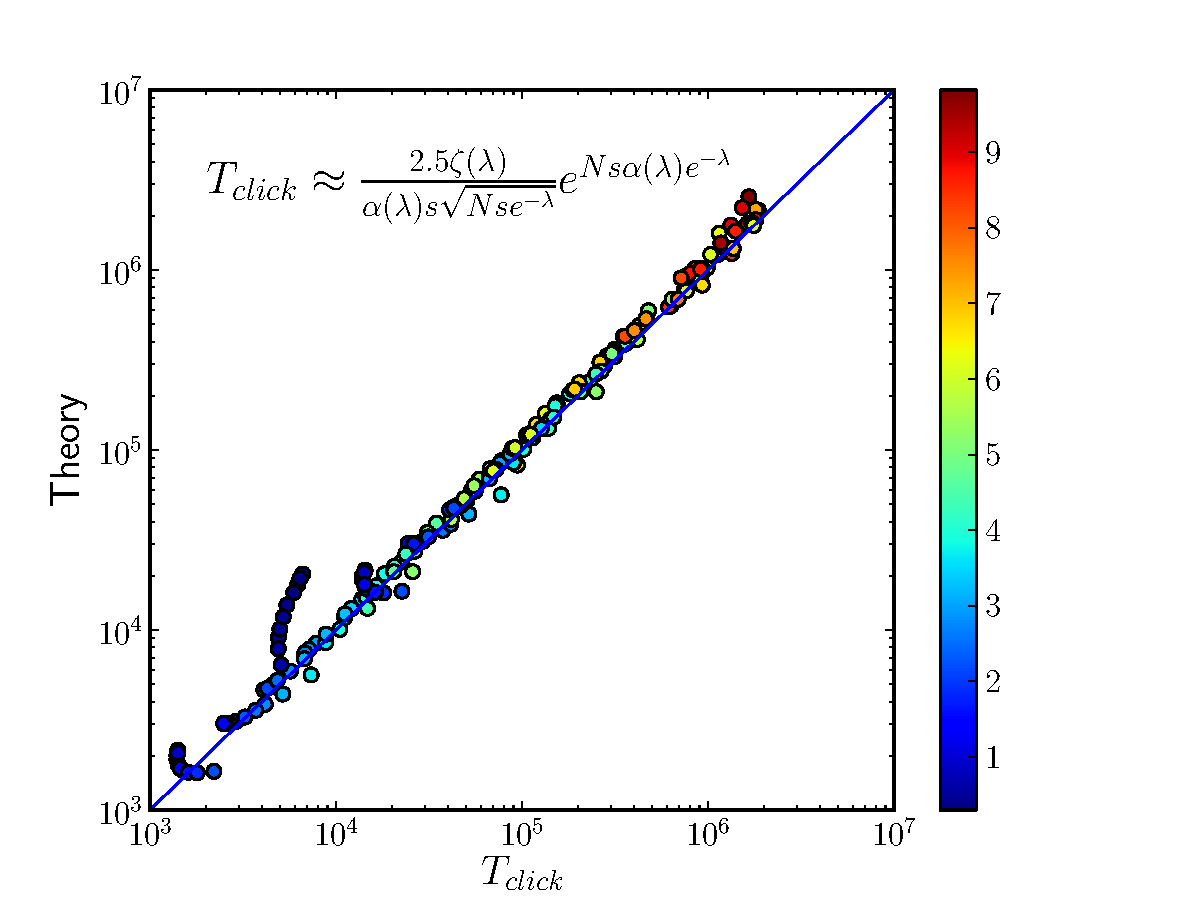
\includegraphics[width=0.7\columnwidth]{Figures/explicit_theory_simulation_comparison.pdf}
  \caption[labelInTOC]{The approximation of the mean time between clicks of the ratchet is accurate over a large range of parameters if $Ns\alpha(\lambda)e^{-\lambda}$ is large compared to one. $Ns\alpha(\lambda)e^{-\lambda}$ determines whether the clicks of the ratchet are far apart compared to the relaxation time of the distribution and is indicated as the color of the data points. The condition  $Ns\alpha(\lambda)e^{-\lambda}>1$ is violated for the fastest clicks shown, resulting in the deviation of the dark blue points.}
  \label{fig:explicit}
\end{center}
\end{figure}

\bibliography{bib}
\end{document}